\documentclass[conference]{IEEEtran}
\IEEEoverridecommandlockouts
\usepackage[T1]{fontenc}
\usepackage{amsmath,amssymb}
\usepackage{graphicx}
\usepackage{booktabs}
\usepackage{url}
\usepackage[hidelinks]{hyperref}
\graphicspath{{figures/}}
\title{Traffic Timing Assistant: Decision-Tree Plan Selection with ARM--FPGA Execution Feedback}
\author{\IEEEauthorblockN{Po Sheng Wei}
\IEEEauthorblockA{IoT Data Analysis and Applications\\National Chung Hsing University, Taiwan}
\thanks{DIC4 individual coursework draft, 25 November 2026. Based on the Group 13 Traffic Assistant project and its preserved DIC3 records. This manuscript reports an audit of archived evidence; no new model training, traffic simulation, or hardware experiment was performed for DIC4.}}
\begin{document}
\maketitle

\begin{abstract}
An adaptive signal-control prototype must connect a traffic-dependent recommendation to evidence that the selected timing plan actually took effect. This paper presents Traffic Timing Assistant, a single-intersection educational system that combines a compact decision-tree policy on an ARM processor with cycle-boundary plan adoption on an FPGA. Four integer features summarize estimated queues and arrivals in the preceding complete 30-second window. The policy selects among three predefined green-time allocations and retains a reference-rule fallback outside its supported domain. Execution readback distinguishes a submitted plan from an applied plan. We reconstruct and audit the existing project evidence rather than report new experiments. Across 18 archived paired synthetic cases, aggregate queue vehicle-seconds decrease from 399,954 under fixed balanced timing to 326,830 under the tree-plus-fallback policy, a reduction of 18.28\%; however, five cases regress. A separately packaged six-case record is identified as the same seed subset and is not treated as independent replication. An archived board report describes one paired execution, while its underlying raw traces are absent from the current handoff. Reproducible arithmetic checks, OpenSpec requirements, and a read-only Model Context Protocol workflow make these evidence boundaries explicit. The result is a reviewable course prototype and evaluation artifact; effectiveness on real roads and a benefit over the labeling rules remain unestablished.
\end{abstract}
\begin{IEEEkeywords}
traffic signal control, decision trees, ARM, FPGA, execution feedback, evidence provenance
\end{IEEEkeywords}

\section{Introduction}
Traffic signals allocate a limited service opportunity among conflicting movements. A fixed allocation can become poorly matched to directional demand, yet a change in recommended timing is only one part of an operational control chain. The traffic input must be interpretable, a legal plan must be selected, and the device must apply that plan at the intended boundary. Standard signal-timing guidance treats green intervals, change intervals, and clearance intervals as distinct design elements whose values depend on the application \cite{koonce2008timing}.

The Traffic Assistant project addresses these concerns in a deliberately bounded teaching setting: one intersection, two through-traffic axes, three timing plans, and an existing ARM--FPGA prototype. Its four-feature decision tree approximates a rule-based plan scorer. The ARM maintains synthetic FIFO queue state and selects a plan; the FPGA preserves the phase order and adopts pending plans at complete cycle boundaries. The application therefore exposes three different observations: a recommendation, a submission, and subsequent execution feedback.

This DIC4 draft develops the earlier proposal into a conference-style description, grounded in the preserved source snapshot and result records \cite{projectdesign,projecthost,projectreport}. It addresses three questions. \emph{RQ1:} under the archived inputs, which scenarios improve or regress relative to fixed timing? \emph{RQ2:} what evidence distinguishes model selection, fallback, and actual plan adoption? \emph{RQ3:} which findings can be rechecked from the available handoff, and which require missing inputs or hardware traces?

The contributions are a bounded system description with an explicit plan-adoption contract; a reproducible reanalysis of saved paired results, including regressions and overlapping records; and a specification-backed artifact workflow connecting claims to their sources. These contributions concern an educational implementation and evidence management. The draft does not propose a new traffic-control optimality theorem or assert that the complete planned task interface has already been integrated.

\section{Related Work}
\subsection{Learning and Interpretable Timing Decisions}
Tariq \emph{et al.} combine recursive partitioning and regression trees with fuzzy rules to learn timing experts' responses during non-recurrent congestion \cite{tariq2020signal}. Their work supports the relevance of learning structured green-time decisions, but uses historical expert behavior and a different control formulation. Our prototype instead uses a deterministic scorer to label a three-action classification problem.

Ault \emph{et al.} study interpretable polynomial control functions trained with reinforcement-learning techniques \cite{ault2020interpretable}. Their results motivate human-inspectable policies without implying that their polynomial policy, training procedure, or performance transfers to this decision tree. VIPER extracts tree policies using an oracle neural policy and its action-value information, then analyzes properties on specified control tasks \cite{bastani2018viper}. Here, neither VIPER training nor formal verification has been performed. A tree representation alone establishes neither correctness nor a traffic-performance guarantee.

\subsection{Evaluation and Project Position}
The archived 2008 FHWA manual provides background on timing parameters and evaluation \cite{koonce2008timing}; it is not used as current local compliance guidance. SUMO supplies a richer microscopic simulation environment \cite{lopez2018sumo}, which would support a future evaluation with vehicle movement, intersection geometry, and controlled demand. The present results use the project's simpler FIFO model. No SUMO experiment or direct comparison against the cited learning methods is included.

The project is positioned between plan selection and verifiable embedded execution. Its open integration tasks are data qualification, a structured request interface, and unified explanation and reporting. These are gaps in this particular prototype, rather than evidence that the broader literature lacks such capabilities.

\section{System Design}
\subsection{Bounded Intersection and Timing Plans}
Let the two movement axes be north--south (NS) and east--west (EW). Table~\ref{tab:plans} lists the entire action space. Each plan uses the phase order NS green, NS yellow, all red, EW green, EW yellow, all red. The two yellow intervals are 2~s each and the two all-red intervals are 1~s each. Thus,
\begin{equation}
 C=g_{\mathrm{NS}}+g_{\mathrm{EW}}+2(2+1)=30\ \mathrm{s}.
\end{equation}
These are documented desktop-demo parameters, not calibrated road timings. Plan changes leave the active phase and countdown intact and take effect at a complete cycle boundary \cite{projectdesign}.

\begin{table}[t]
\caption{Complete action space of the preserved prototype.}
\label{tab:plans}
\centering
\begin{tabular}{clrr}
\toprule
Plan ID & Meaning & NS green (s) & EW green (s)\\
\midrule
0 & Balanced & 12 & 12\\
1 & NS priority & 16 & 8\\
2 & EW priority & 8 & 16\\
\bottomrule
\end{tabular}
\end{table}

\begin{figure*}[t]
\centering
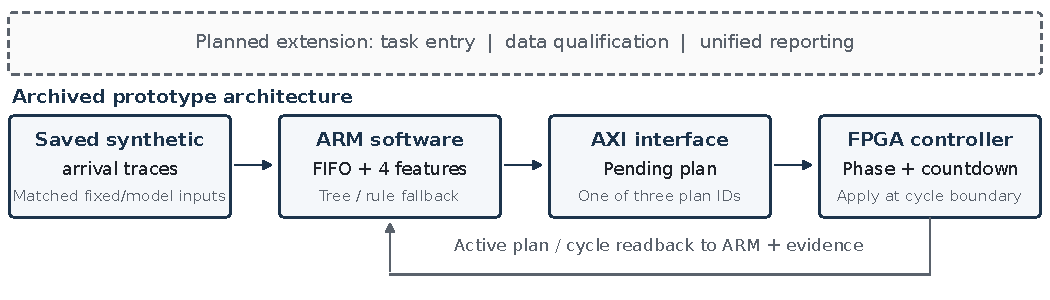
\includegraphics[width=0.96\textwidth]{architecture.pdf}
\caption{Documented control core and its planned task-level extension. The ARM updates estimated queues and selects a pending plan; the FPGA controls phases and exposes readback. Dashed elements remain integration work. MCP is used in the separate authoring/evidence workflow, not in this real-time control loop.}
\label{fig:architecture}
\end{figure*}

\subsection{Features, Tree, and Rule Fallback}
At a decision boundary, the feature vector is
\begin{equation}
 x=[q_{\mathrm{NS}},q_{\mathrm{EW}},a^{30}_{\mathrm{NS}},a^{30}_{\mathrm{EW}}],
\end{equation}
where $q$ is the current estimated FIFO length after the observed update and $a^{30}$ counts arrivals in the preceding complete 30-second window. These queue values are software states, not measured road queues. The preserved model header identifies 513 nodes and maximum depth 10; the archived validation record reports a 4,104-byte model representation. Its declared domain is $0\leq q_d\leq120$ and $0\leq a^{30}_d\leq30$ for each axis $d$. The per-second arrival interface accepts only 0 or 1 per axis \cite{projectdesign,projecthost}.

The source scorer rolls each candidate plan forward over one cycle using a constant arrival rate estimated from that window. To retain exact rational arithmetic, its queue state is scaled by 30. If $s_d^p(h)$ is 1 when plan $p$ serves axis $d$ at future second $h$, and 0 otherwise, its update is
\begin{align}
 z_d^p(0)&=30q_d,\\
 z_d^p(h)&=\max\{0,z_d^p(h-1)+a^{30}_d-30s_d^p(h)\},\\
 J_p&=\sum_{h=1}^{30}\big(z_{\mathrm{NS}}^p(h)+z_{\mathrm{EW}}^p(h)\big).
\end{align}
The update is evaluated for $h=1,\ldots,30$, and $J_p/30$ is the predicted QVS. The minimum-cost plan supplies the reference decision, with the earlier plan ID retained on a tie. The scorer's fluid prediction differs from the discrete, observed FIFO updates used for evaluation. The tree learns this scorer's labeling rule; it does not independently learn a real-road reward.

The preserved firmware policy uses the tree within its domain and the reference rule when outside the domain or when an invalid model output is detected. An inspection of the preserved C source also shows that all three rule costs are computed before policy selection. Consequently, this implementation does not establish that tree selection eliminates rule computation or provides an inference-time speedup. A latency or energy comparison would require a separate measurement.

\subsection{Recommendation, Submission, and Adoption}
Fig.~\ref{fig:architecture} separates processor-side selection from FPGA execution. After each complete observation window, the ARM forms features, records the decision source, and submits a legal pending plan through the documented AXI path. The FPGA retains the current phase durations until the next complete cycle, then updates the active plan. A meaningful execution record links the submitted plan to the subsequently observed active plan and cycle count. Submission alone cannot establish adoption.

The source snapshot supports checks for phase range, plan range, remaining duration, and coherent state progression. The archived board report additionally describes readback-based verification \cite{projectreport}. The complete RTL, executable firmware build, and raw board captures are not contained in this DIC4 handoff; those historical execution claims therefore retain their original evidence level.

\subsection{Data Qualification and Remaining Integration}
The proposed task layer records a data identifier, mode, units, time coverage, and directional provenance before control. Minute-resolution official observations cannot simply be relabeled as per-second measurements. A missing minute must remain missing, and unrelated directions cannot be paired without justification. The earlier project identified insufficient continuous two-axis official input and used saved synthetic scenarios for control comparisons \cite{projectdesign}.

The OpenSpec change for task integration remains pending. Its acceptance scenarios include insufficient-data rejection, out-of-domain fallback, review-only operation, and submitted-versus-applied reporting. The specification describes intended behavior; passing its structural validation does not establish that the application behavior is implemented.

\section{Evidence and Evaluation Method}
\subsection{Archived Records and Current Reanalysis}
Table~\ref{tab:evidence} separates the evidence available for this draft. The 18 paired cases consist of six named synthetic scenarios and three seed identifiers, with 600 observations per run. They are extracted from 54 archived policy summaries, which also include the reference-rule policy \cite{projecthost}. Fixed balanced timing and tree plus fallback form the primary comparison. The report documents the same initial queues, cycle settings, and service assumptions for paired runs.

The DIC4 audit reloads the summaries, recalculates totals and percentages, checks vehicle conservation, checks decision counts, detects the overlap of the six-case package, and compares snapshot hashes against the preserved manifest. It performs 164 checks. It does not regenerate input vectors, execute the original firmware, retrain the model, or reacquire board samples. Therefore, internal record consistency and historical execution provenance are distinct conclusions.

\begin{table*}[t]
\caption{Evidence levels in the current handoff. Historical records are kept distinct from checks executed for DIC4.}
\label{tab:evidence}
\centering\small
\begin{tabular}{p{0.18\textwidth}p{0.37\textwidth}p{0.36\textwidth}}
\toprule
Evidence item & Available material & Conclusion supported here\\
\midrule
18 paired host cases & Archived JSON with 54 policy summaries and source identities & Current recalculation and consistency checks of reported outcomes; no fresh firmware execution\\
6-case host package & Detailed comparison JSON for seed 2779054081 & Scenario-level inspection; the same seed subset of the 18-case record, not an additional sample\\
One paired board case & Archived experiment narrative and its reported result table & Description of the historical board report; raw traces and independent revalidation unavailable\\
Source snapshot & Design document, engine C file, model header, and manifest & Inspection of documented plans, features, fallback, and scoring logic; full build is unavailable\\
DIC4 artifacts & Audit outputs, OpenSpec logs, MCP run record, LaTeX sources & Reproducible document/evidence workflow, with online publication status reported separately\\
\bottomrule
\end{tabular}
\end{table*}

\subsection{Metrics and Comparison Rules}
Let $q_d(t)$ denote the queue remaining after arrivals and service at observation $t$. The primary metric is queue vehicle-seconds (QVS):
\begin{equation}
 V=\sum_{t=0}^{599}\big(q_{\mathrm{NS}}(t)+q_{\mathrm{EW}}(t)\big)\Delta t,
 \qquad \Delta t=1\ \mathrm{s}.
\end{equation}
For a set $S$ of paired cases, the reported relative change is
\begin{equation}
 \Delta_V(S)=100\left(\frac{\sum_{i\in S}V_i^{\mathrm{tree+fallback}}}
 {\sum_{i\in S}V_i^{\mathrm{fixed}}}-1\right)\%.
\end{equation}
A negative value means less queue burden. This is a ratio of sums, not the mean of per-case percentages. Completed-vehicle mean waiting time, departures, residual NS/EW queues, and fallback counts provide complementary information. In particular, a low mean wait among completed vehicles can coexist with a large queue still waiting at the end.

The 600-observation window is fixed. After observation 599, the twentieth decision still awaits adoption. The historical host validator compares 19 applied decisions per case and checks the final unused decision separately \cite{projecthost}. The archived board report describes confirmation of the twentieth adoption outside the traffic-performance window while arrivals, service, and QVS remain frozen \cite{projectreport}. Continuing to drain queues would change the experiment and is excluded by this contract.

\section{Results and Interpretation}
\subsection{Aggregate and Scenario-Level Outcomes}
The recalculated 18-case total is 399,954 QVS for fixed balanced timing and 326,830 QVS for tree plus fallback, yielding $\Delta_V=-18.2831\%$. Thirteen cases improve and five regress. The largest recorded regression is the bursty case with seed 2779054082: 2,881 to 3,517 QVS, an increase of 22.08\%. Fig.~\ref{fig:changes} displays every case rather than hiding these regressions in the total.

\begin{figure}[t]
\centering
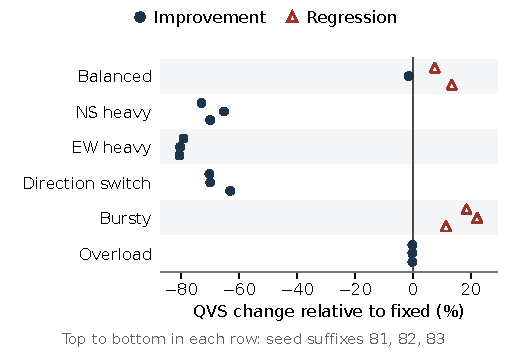
\includegraphics[width=\columnwidth]{scenario_changes.pdf}
\caption{Recalculated changes for all 18 archived pairs. Each marker is one saved seed within a scenario. Negative values mean lower QVS than fixed balanced timing; positive values are regressions. These are descriptive results from the preserved summaries.}
\label{fig:changes}
\end{figure}

Table~\ref{tab:six} provides the detailed six-case view for seed 2779054081. Its total reduction is 19.71\%, but the balanced and bursty cases worsen. During overload, both policies release 475 of 781 arrivals, leaving 306 vehicles. Residual NS/EW queues change from 155/151 to 79/227. Thus the small total-QVS reduction accompanies a more uneven directional backlog. This case motivates reporting both axes and unfinished demand.

\begin{table}[t]
\caption{Detailed archived subset, seed 2779054081. QVS units are vehicle-seconds; $\Delta$ is relative to fixed timing.}
\label{tab:six}
\centering\small
\begin{tabular}{lrrr}
\toprule
Scenario & Fixed & Tree+fallback & $\Delta$ (\%)\\
\midrule
Balanced & 3,035 & 3,263 & +7.51\\
NS heavy & 11,815 & 3,202 & $-72.90$\\
EW heavy & 14,972 & 3,126 & $-79.12$\\
Direction switch & 10,369 & 3,089 & $-70.21$\\
Bursty & 3,485 & 4,126 & +18.39\\
Overload & 93,817 & 93,589 & $-0.24$\\
\midrule
Total & 137,493 & 110,395 & $-19.71$\\
\bottomrule
\end{tabular}
\end{table}

The six rows match the corresponding archived seed within the 18-pair record. They are a detailed view of existing cases and are never pooled to claim 24 independent tests. The three seed identifiers themselves also do not establish a calibrated road-demand distribution or a statistical significance result.

\subsection{Fallback and the Labeling Reference}
Across the 18 model-policy runs, the summaries contain 329 tree decisions and 31 rule fallbacks. In the six-case subset, these counts are 110 and 10. The policy-level comparison therefore includes both mechanisms. Attributing every improvement solely to the tree would be unsupported.

For context, the same archived file reports 326,533 QVS for direct reference-rule selection, compared with 326,830 for tree plus fallback: the tree policy is 297 QVS, or about 0.091\%, higher in aggregate. This is a reanalysis of the preserved third-policy records, not a newly run baseline. It provides no evidence that the tree improves on its labeling reference. Any future claim of deployment advantage must measure an actual benefit, such as implementation cost or decision latency, under an appropriate implementation and common conditions.

\subsection{Historical Execution Report}
The archived experiment narrative records a direction-switch board pair with 361 synthetic arrivals in each run, fixed/model departures of 331/359, and QVS of 10,369/3,089. It reports 20 submissions and 20 adoption confirmations per run, with the last confirmation outside the fixed performance window \cite{projectreport}. The traffic metrics were calculated by the ARM's simplified FIFO model while FPGA phases determined service opportunities. They were not road-sensor measurements.

Only the report and its summary are available in this handoff; the linked raw mailbox captures and board-verification files are absent. The DIC4 work checks the table's arithmetic and conservation, but does not independently verify those past hardware executions. According to the archived report, the board pair reuses the direction-switch input described in the detailed host subset. It is an execution-consistency example, not another independent demand trial.

\section{Reproducible Artifact Workflow}
The repository separates immutable archived inputs from current derived outputs. A Python audit regenerates the JSON summary and per-case CSV tables; the plotted values come directly from that summary. A claim-to-source table identifies the files supporting quantitative and architectural statements. The paper uses the official IEEE conference class with editable LaTeX and bibliographic sources.

OpenSpec 2.0.0 \cite{openspec} preserves the earlier control and evaluation specifications, retains the unfinished task-integration change, and adds a conference-draft change. Strict validation covers three main specifications and two active changes. The planning-artifact status is kept separate from task completion and actual online publication.

The Model Context Protocol (MCP) defines an interface between AI applications and external tools or data \cite{mcp}. In this assignment, a read-only local MCP server exposes the evidence inventory, audit summary, and design excerpt. A real stdio client initializes the server, discovers three tools, and retrieves their outputs using the official Python SDK. All 14 workflow checks pass, including an independent recalculation of the archived totals against the returned summary. The saved responses and execution metadata supply a repeatable authoring/provenance demonstration. This workflow is outside the traffic controller; Overleaf and GitHub publication have separate status records.

\section{Limitations and Next Steps}
The current study is limited to two through-traffic axes, three fixed plans, a 30-second cycle, and a discrete FIFO service abstraction. It omits geometric calibration, turning flows, pedestrian phases, vehicle dynamics, and measured emissions. Synthetic summaries support comparisons within their stated assumptions. The available source subset cannot reproduce the original full firmware build or independently rerun the archived traffic experiment.

The next implementation step is the pending structured task interface with source qualification and unified execution reporting. The next evidence step is to recover the complete model implementation, saved arrival vectors, manifests, and raw board traces. A subsequent experiment should use held-out demand sequences, report per-direction residual queues and variability, and compare fixed timing, the reference rule, and the tree policy under the same inputs. SUMO-based evaluation is a possible later extension after the input model and comparison protocol are defined \cite{lopez2018sumo}.

\section{Conclusion}
Traffic Timing Assistant connects a constrained learned plan selector to explicit ARM--FPGA execution feedback. Reanalysis of 18 archived pairs confirms an 18.28\% aggregate QVS reduction relative to fixed balanced timing while preserving five regressions, fallback use, and the limits of the reference-rule comparison. The six-case package is an overlapping subset, and the historical board claim remains report-level evidence in this handoff. The conference draft, reproducible audit, OpenSpec specifications, and executed MCP workflow provide a concrete basis for review and further implementation without overstating traffic effectiveness or validation completeness.

\bibliographystyle{IEEEtran}
\bibliography{references}
\end{document}
